%%%%%%%%%%%%%%%%%%%%%%%%%%%%%%%%%%%%%%%%%%%%%%%%%%%%%%%%%%%%%%%%%%%%%%%%%%% 
% 
% Generic template for TFC/TFM/TFG/Tesis
% 
% By:
% + Javier Macías-Guarasa. 
% Departamento de Electrónica
% Universidad de Alcalá
% + Roberto Barra-Chicote. 
% Departamento de Ingeniería Electrónica
% Universidad Politécnica de Madrid   
% 
% Based on original sources by Roberto Barra, Manuel Ocaña, Jesús Nuevo,
% Pedro Revenga, Fernando Herránz and Noelia Hernández. Thanks a lot to
% all of them, and to the many anonymous contributors found (thanks to
% google) that provided help in setting all this up.
% 
% See also the additionalContributors.txt file to check the name of
% additional contributors to this work.
% 
% If you think you can add pieces of relevant/useful examples,
% improvements, please contact us at (macias@depeca.uah.es)
% 
% You can freely use this template and please contribute with
% comments or suggestions!!!
% 
%%%%%%%%%%%%%%%%%%%%%%%%%%%%%%%%%%%%%%%%%%%%%%%%%%%%%%%%%%%%%%%%%%%%%%%%%%% 

\chapter{Theoretical Background}
\label{cha:theoretical_background}

\begin{FraseCelebre}
	\begin{Frase}
		Desde que el mundo cambió, estamos mucho más unidos \\
		con los Digimon, luchamos juntos contra el mal. \\ 

		Algo extraño pasaba, Digievolucionaban, \\
		en tamaño y color, ellos son los Digimon. \\
	\end{Frase}
	\begin{Fuente}
		Opening 1 de Digimon: "Butterfly" \\
		Autor original: Kōji Wada
	\end{Fuente}
\end{FraseCelebre}

\section{Introduction}
\label{sec:3_introduction}

As commented in previous sections, the \ac{MP} algorithms covered by this thesis range from tracking multiple objects and subsequent prediction with physics-based methods to the most recent \ac{SOTA} techniques to compute the deep traffic context and then decode multimodal predictions with associated confidences, assuming the physical information is given and surrounding participants have been multi-tracked beforehand. Throughout this Chapter, an in-depth theoretical study will be made of those algorithms, neural networks or heuristics that form a direct part of the development of this work in order to address the proposed methods in Chapter \ref{cha:predictive_techniques}. \\

First of all, we will start with the mathematical formulation of the methods to perform physics-based Multi-Object Tracking, from the well-known techniques Kalman Filter \cite{kalman1960new} for the agents states estimation to the Hungarian algorithm \cite{kuhn1955hungarian} for the association of detections and trackers, which represents the preliminary stage before carrying out the subsequent prediction. On top of that, since several single-trajectory models (\ac{CTRV}, \ac{CTRA}) are used to compute the most plausible centerlines in the Argoverse 1 \cite{chang2019argoverse} and Argoverse 2 \cite{wilson2023argoverse}, we will review the state transition equations to properly understand the constraints for each model. Furthermore, the principal \ac{DL} techniques (e.g. 1D-CNN, LSTM, GCN, Attention mechanisms) and training losses used in this work to encode and decode the aimed multimodal will be stated, first a general mathematical formulation and applications and then how the corresponding technique is used in the \ac{MP} field.

\section{Physics-based algorithms}
\label{sec:3_pb_formulation}

% https://arxiv.org/pdf/1710.04055.pdf
% https://github.com/NickNair/Multiple-Object-Tracking-using-Kalman-Filter

As stated in Chapter \ref{cha:related_works} Section \ref{sec:2_introduction}, initially researchers rely on physics-based methods which are basic and straightforward. These methods may not offer high accuracy, but many models use the underlying idea of physics-based models to improve their accuracy. Physics-based approaches yield better results when the movement of vehicles is described by kinematics or dynamics models accurately. Nevertheless, the physical model of traffic participants is constantly evolving, so most physics-based models are only applicable for short-term predictions of no more than one second. In this Section we will study the mathematical formulation of the physics-based prediction algorithms, as well as the data association problem regarding the Multi-Object Tracking stage, that are directly related to our algorithms proposed in Chapter \ref{cha:predictive_techniques}.

\subsection{Kalman Filter under the hood}
\label{subsec:3_kf_formulation}

The Kalman Filter \cite{kalman1960new} is a recursive algorithm used for estimating the state of a dynamic system in the presence of noise. It is widely used in various fields such as engineering, control systems, and robotics. The algorithm works by combining a prediction of the system state based on a mathematical model with measurements (updates) from sensors to improve the accuracy of the state estimation, as shown in Figure \ref{fig:3_KF_cycle}. The Kalman Filter is a powerful algorithm for state estimation, and it has many variations and extensions that can handle various types of systems and measurements. The filter can be applied to non-linear systems using the Extended Kalman Filter or the Unscented Kalman Filter, and it can handle multiple models using the multiple model Kalman Filter. The filter can also be used for smoothing, which involves estimating the state of the system based on past and future measurements.

\begin{figure}[h]
	\centering
	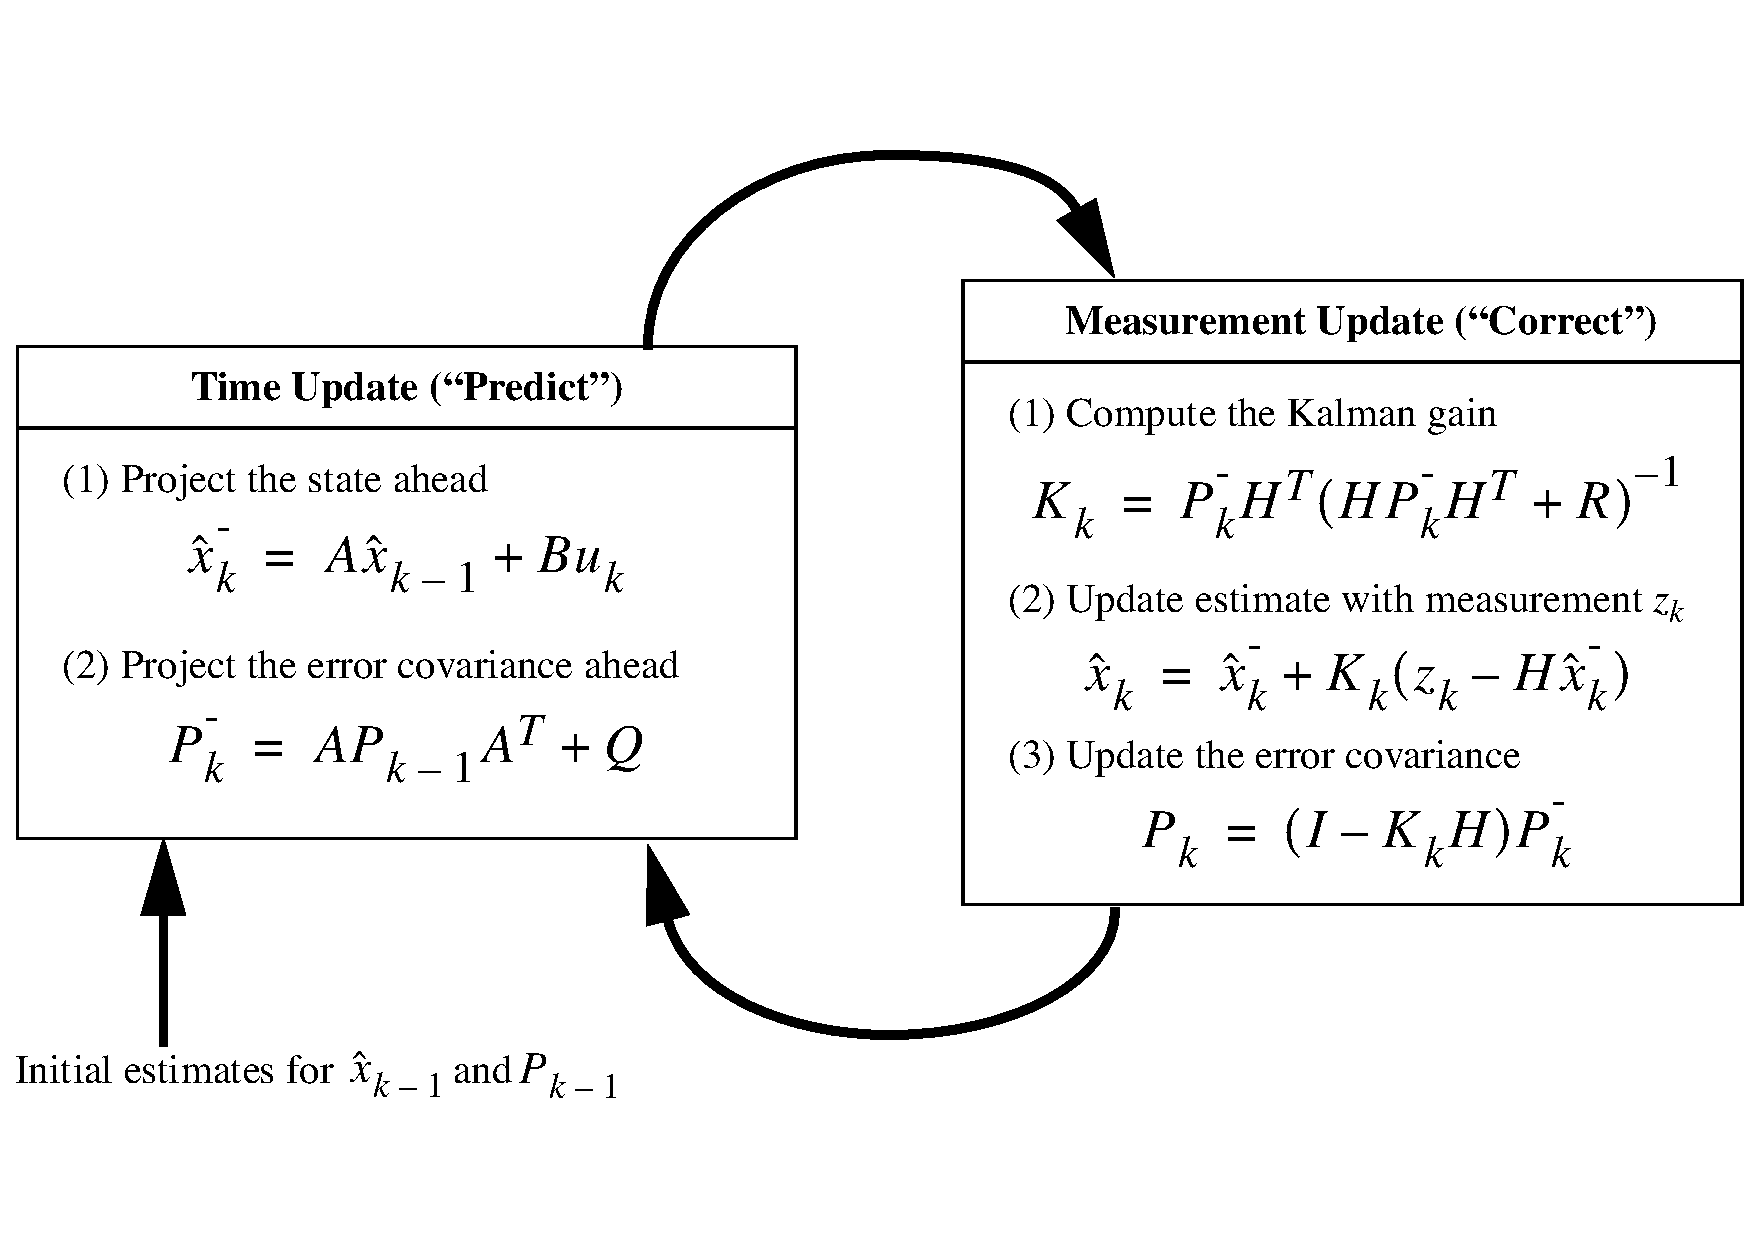
\includegraphics[width=\linewidth]{3_KF_cycle.pdf}
	\caption[Overview of the Kalman Filter Predict-Update cycle]{Overview of the Kalman Filter Predict-Update cycle. The Kalman filter keeps track of the estimated state of the system and the variance or uncertainty of the estimate. The estimate is updated using a state transition model and measurements}
	Source: \textit{An introduction to the kalman filter} \cite{bishop2001introduction}
	\label{fig:3_KF_cycle}
\end{figure}

In its most simple version, the Kalman filter assumes that the system can be described using a set of linear equations, where the state of the system can be represented by a vector $\mathbf{x}_k$, and the measurements can be represented by a vector $\mathbf{z}_k$. The Kalman filter also assumes that the noise in the system follows a Gaussian distribution.

The state estimation process is performed in two steps: the prediction step and the update step. In the prediction step, the current state of the system is predicted based on the previous state and a mathematical model of the system. In the update step, the predicted state is corrected based on a measurement from a sensor.

The prediction step can be represented using the following equations:

\begin{equation}
\begin{split}
	\hat{\mathbf{x}}_k^- = \mathbf{A} \hat{\mathbf{x}}_{k-1} + \mathbf{B} \mathbf{u}_k \\
	\mathbf{P}_k^- = \mathbf{A} \mathbf{P}_{k-1} \mathbf{A}^T + \mathbf{Q}
\end{split}
\end{equation}

where $\hat{\mathbf{x}}_k^-$ is the predicted state of the system at time $k$, $\hat{\mathbf{x}}_{k-1}$ is the estimated state of the system at time $k-1$, $\mathbf{A}$ is the state transition matrix, $\mathbf{B}$ is the control-input matrix, $\mathbf{u}_k$ is the control input at time $k$, $\mathbf{P}_k^-$ is the predicted error covariance matrix, and $\mathbf{Q}$ is the process noise covariance matrix. Note that the state transition, control-input and process noise covariance matrix values do not depend on the timestep time $k$.

On the other hand, the update step can be represented using the following equations:

\begin{equation}
	\begin{split}
		\mathbf{K}_k = \mathbf{P}_k^- \mathbf{H}_k^T (\mathbf{H} \mathbf{P}_k^- \mathbf{H}^T + \mathbf{R})^{-1} \\
		\hat{\mathbf{x}}_k = \hat{\mathbf{x}}_k^- + \mathbf{K}_k (\mathbf{z}_k - \mathbf{H}_k \hat{\mathbf{x}}_k^-) \\
		\mathbf{P}_k = (\mathbf{I} - \mathbf{K}_k \mathbf{H}) \mathbf{P}_k^-
	\end{split}
\end{equation}

where $\mathbf{K}_k$ is the Kalman gain, $\mathbf{H}$ is the measurement matrix, $\mathbf{R}_k$ is the measurement noise covariance matrix and $\mathbf{I}$ the identity matrix of the corresponding dimension. The Kalman gain determines the relative weight given to the predicted state and the measurement, and is adjusted based on the measurement noise covariance matrix. The measurement matrix relates the measurements to the state variables, and is used to convert the measurements into the same units as the state variables.

\subsection{Hungarian algorithm formulation}
\label{subsec:3_HA_formulation}

The Hungarian algorithm \cite{kuhn1955hungarian}, also known as the Munkres algorithm or the Kuhn-Munkres algorithm, is an efficient algorithm for solving the assignment problem in combinatorial optimization. The main concept behind this algorithm is an assignment problem that involves finding the optimal assignment of $n$ workers to $n$ jobs, given the cost of assigning each worker to each job.

The Hungarian algorithm works by iteratively finding a set of independent zero-cost assignments, which correspond to a perfect matching in a bipartite graph. These assignments are then used to reduce the problem size and find a new set of independent zero-cost assignments, until all workers are assigned to jobs.

The Hungarian algorithm has a time complexity of O($n^3$), which makes it one of the most efficient algorithms for solving the assignment problem. In this algorithm, the cost matrix C is assumed to be an $n \times n$ matrix, where each element $C_{i,j}$ represents the cost of assigning worker i to job j. The matrix M represents the matching, where each element $M_{i,j}$ is 1 if worker i is assigned to job j, and 0 otherwise.

\begin{algorithm}[]
	\SetAlgoLined
	\DontPrintSemicolon
	\SetKwInOut{Input}{Input}
	\SetKwInOut{Output}{Output}
	\Input{A cost matrix $C$ of size $n\times n$}
	\Output{A minimum cost perfect matching}
	Initialize the label vectors $u_i = \min_{j\in{1,\dots,n}} C_{i,j}$ and $v_j=0$ for all $i,j$;
	Initialize the empty matching $M$;
	\While{$|M| < n$}{
		Choose an unmatched row $i$;
		Initialize the set $T = {i}$ and the predecessor vector $P = \emptyset$;
		\While{true}{
			Let $S$ be the set of columns $j$ such that $i\in T$ and $C_{i,j} = u_i + v_j$;
			If $|S| > 0$, choose any column $j$ in $S$;
			\Else{
				Choose a column $j$ such that $v_j = \min_{k\in{1,\dots,n}} v_k$ and let $S$ be the set of rows $i$ such that $j\in M$ or $C_{i,j} = u_i + v_j$;
				Increment each $u_i$ for $i\in T$ by $\delta = \min_{i\in T,j\in S} (u_i+v_j-C_{i,j})$;
				Decrement each $v_j$ for $j\in S$ by $\delta$;
				\For{each row $i\in T$ and each column $j\in S$}{
					\If{$C_{i,j} = u_i+v_j$}{
						Add the edge $(i,j)$ to the alternating tree represented by $M$ and $P$;
						\If{$j$ is unmatched}{
							Augment $M$ along the alternating tree to create a larger matching;
							\Return the updated matching $M$;
						}
						\Else{
							Add $j$ to $T$ and continue the while loop;
						}
					}
				}
			}
		}
	}
	\caption{The Hungarian algorithm for solving the minimum cost perfect matching problem.}
	\label{alg:3_ha}
\end{algorithm}

As observed in Algorithm \ref{alg:3_ha}, the Hungarian algorithm iteratively finds an uncovered zero in the cost matrix C and adds it to the matching M, while also adjusting the cost matrix to ensure that all rows and columns are covered by the matching. This is done by finding the minimum uncovered cost in each row and subtracting it from all uncovered costs in the row, and finding the minimum cost in each uncovered column and adding it to all uncovered costs in the column. Once all rows and columns are covered, the algorithm returns the final matching $M$.

In conclusion, the Hungarian algorithm is a powerful optimization algorithm that solves the assignment problem in polynomial time. The algorithm has a wide range of applications and can be easily adapted to handle various constraints and objectives. The algorithm is also guaranteed to find the optimal solution to the assignment problem, which makes it a valuable tool in many practical settings.
	
\subsection{State Transition Equations of Single-Trajectory Models}
\label{subsec:3_state_transitions_single_traj}

As stated in Chapter \ref{cha:related_works} Section \ref{subsubsec:2_single_trajectory_mp}, Single-trajectory prediction methods are used in the field of motion estimation and control, to predict the future state of an object based on its current state and motion. In these methods, the agents are mostly assumed to comply with motion models that describe their dynamic behavior in such a way these are not able to consider the road-related factors and the uncertainty of the current state is unreliable for long-term prediction. Then, these models should only be used for estimating unimodal trajectories of the surrounding agents in the short-term (no more than 1-s).

\begin{figure}[h]
	\centering
	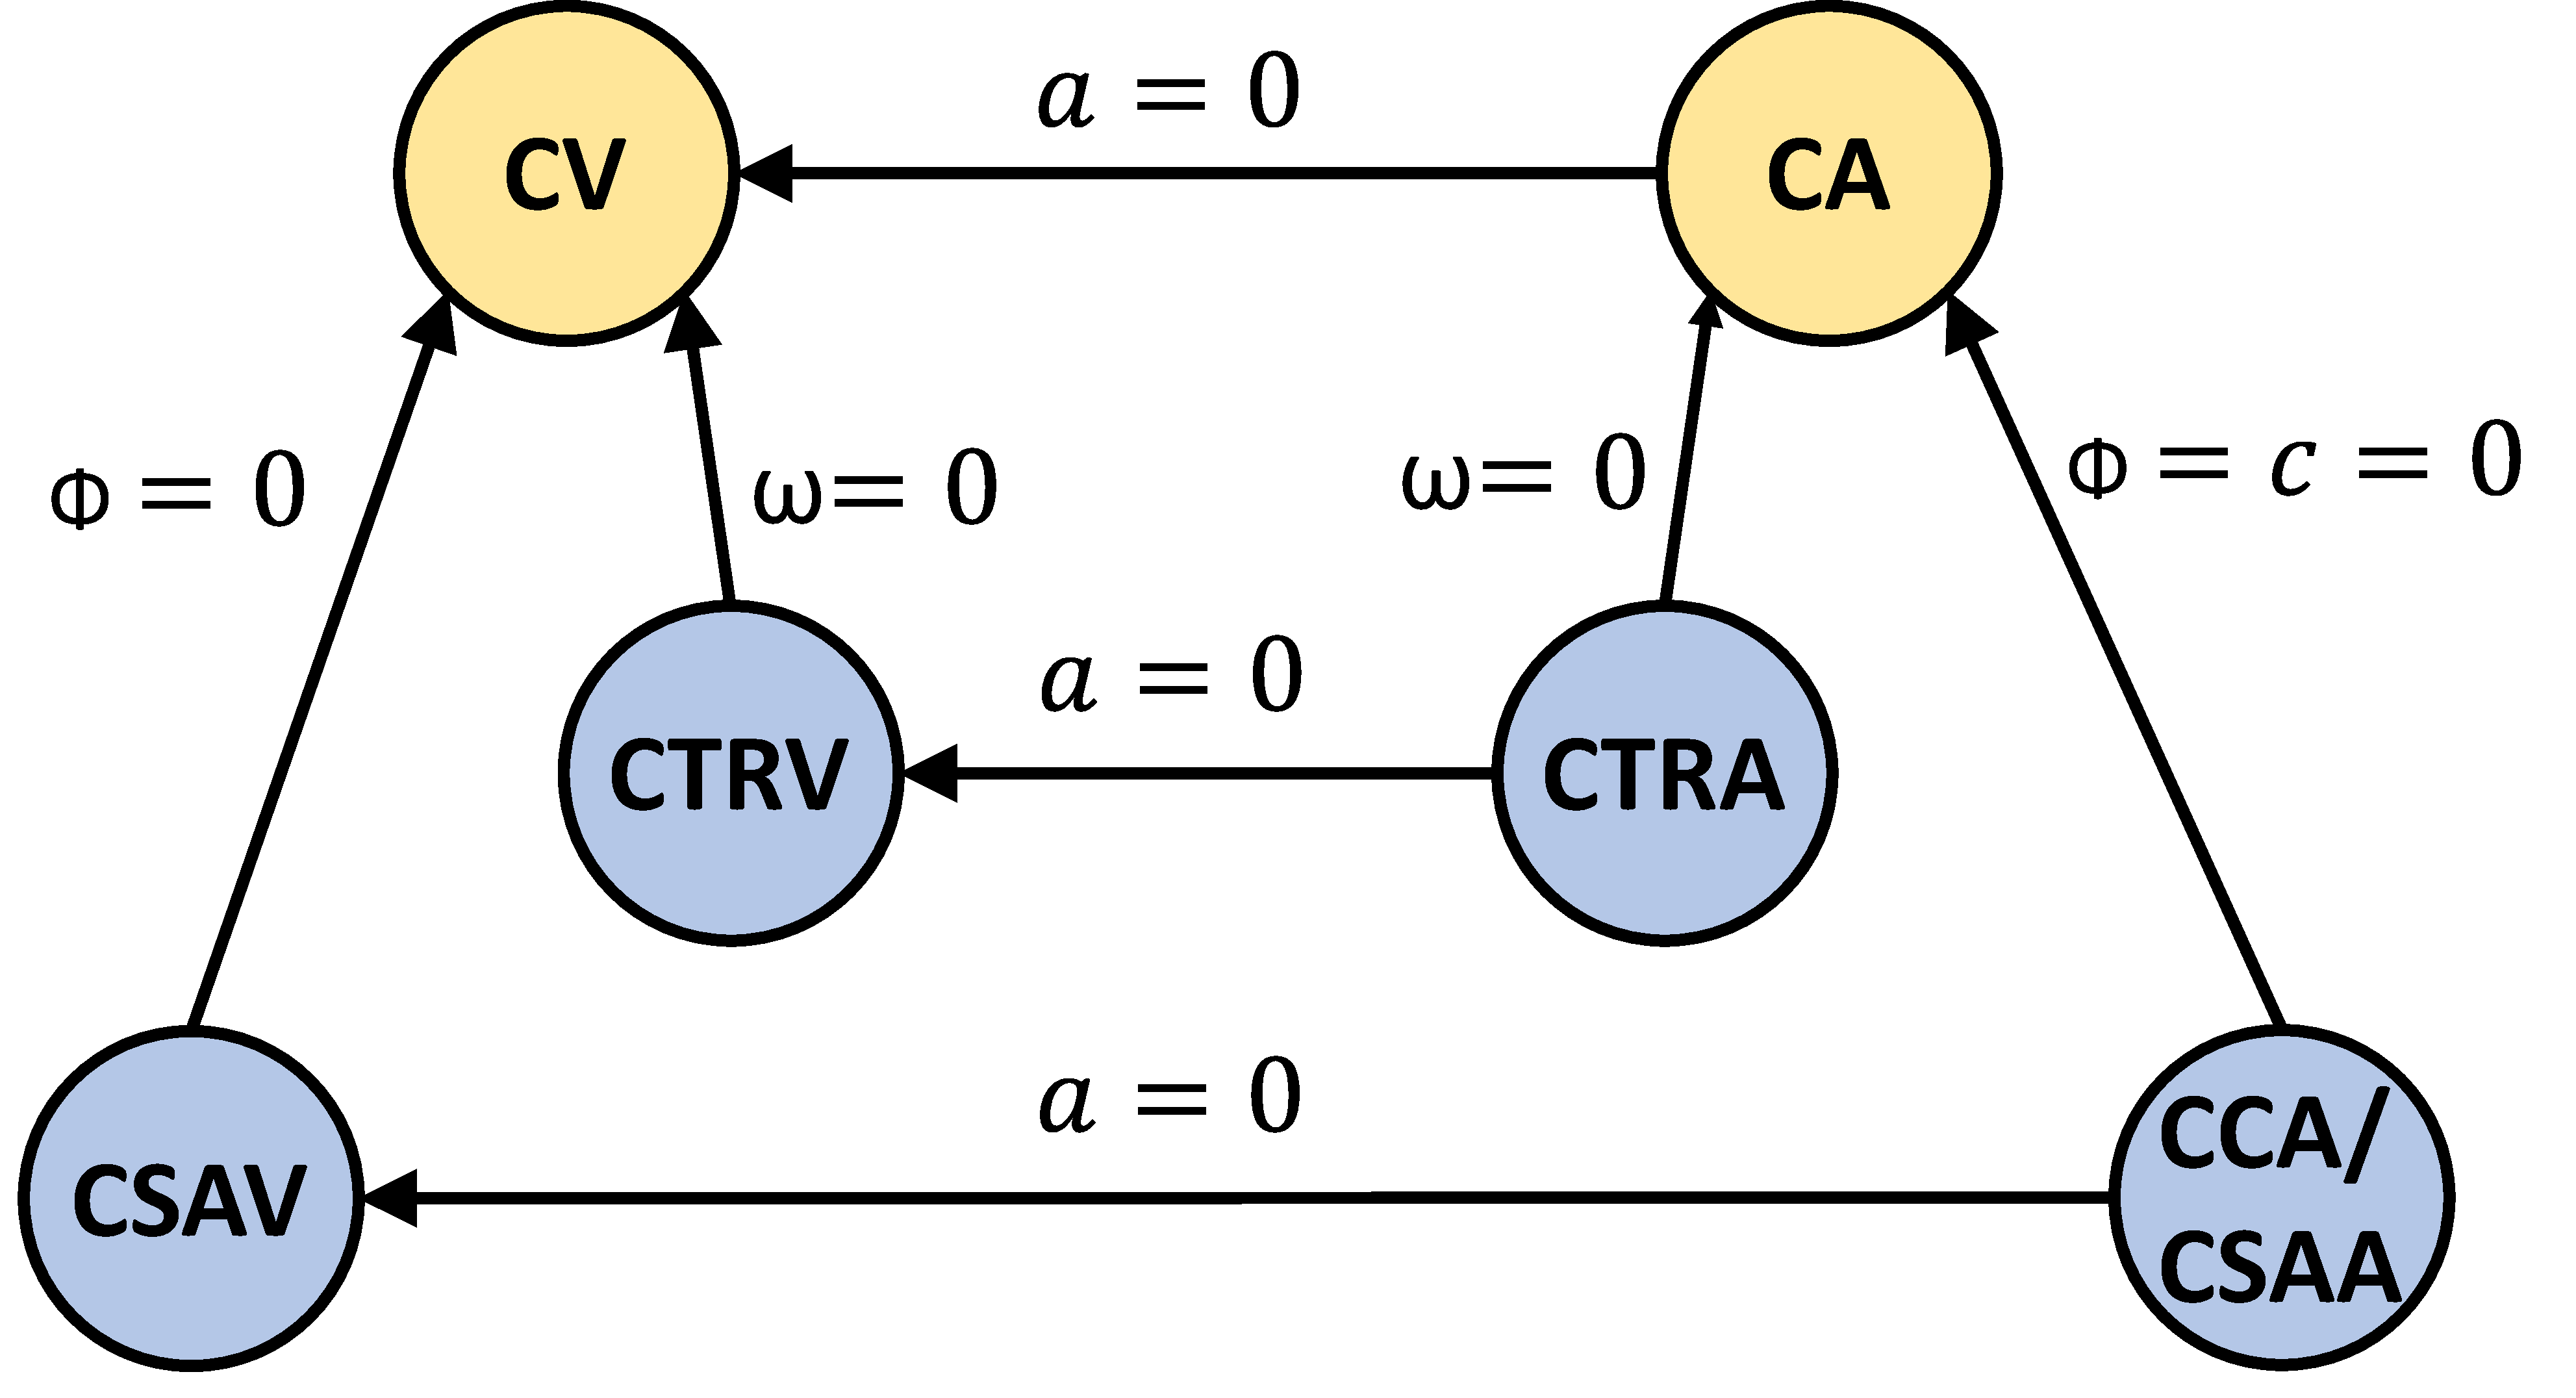
\includegraphics[width=0.6\linewidth]{3_linear_curvilinear_mp.pdf}
	\caption[Overview of Single Trajectory prediction methods]{Overview of Single Trajectory prediction methods. Every sophisticated model can be transformed into a simpler one by setting one state veriable to zero}
	Source: \textit{Comparison and evaluation of advanced motion models for vehicle tracking} \cite{schubert2008comparison}
	\label{fig:3_linear_curvilinear_mp}
\end{figure}

As illustrated in Figure \ref{fig:3_linear_curvilinear_mp}, several single-trajectory prediction models have been proposed in the literature, including Constant Velocity (CV), Constant Acceleration (CA), Constant Turn Rate and Velocity (CTRV), Constant Turn Rate and Acceleration (CTRA), Constant Speed and Angular Velocity (CSAV), and Constant Curvature Acceleration (CCA)/Constant Speed and Angular Acceleration (CSAA). In this Section we focus on the state transition equations of the different methods and how a sophisticated model (e.g. CTRA) can be transformed into a simpler one by setting one state veriable to zero. For example, CTRA is transformed to CTRV if the agent acceleration $a$ is set to zero. Similarly, CTRA is transformed to CA if the angular speed $\omega$ is set to 0.

\subsubsection{Constant Velocity (CV)}
\label{subsubsec:3_CV}

The Constant Velocity (CV) model is a popular single-trajectory prediction model used in the field of motion planning and control. It assumes that the object moves at a constant velocity in a straight line. The state vector of this model includes position and velocity. This means that the position of the object at time $t$ can be calculated by adding the product of the velocity and time to the position at time $t-1$. The velocity at time $t$ is assumed to be the same as the velocity at time $t-1$.

The state vector for the CV model includes position and velocity:

\begin{equation}
	x = \begin{bmatrix}x \\
		               y \\
		               v_x \\
		               v_y
	    \end{bmatrix}
\end{equation}

where $(x,y)$ is the position of the object and $(v_x,v_y)$ is the velocity of the object in the $x$ and $y$ directions, respectively.

The state transition model for the CV model can be written as:

\begin{equation}
	F = \begin{bmatrix}
		 			   1 & 0 & \Delta t & 0 \\
		               0 & 1 & 0 & \Delta t \\
		               0 & 0 & 1 & 0 \\
		               0 & 0 & 0 & 1
		\end{bmatrix}
\end{equation}

where $\Delta t$ is the time step.

The measurement model for the CV model is:

\begin{equation}
	H = \begin{bmatrix}
		1 & 0 & 0 & 0 \\
		0 & 1 & 0 & 0
	    \end{bmatrix}
\end{equation}

which means that the measurements are the position of the object in the $x$ and $y$ directions.

\subsubsection{Constant Acceleration (CA)}
\label{subsubsec:3_CA}

The Constant Acceleration (CA) assumes that the object moves at a constant acceleration in a straight line. The state vector of this model includes position, velocity, and acceleration. This means that the position of the object at time $t$ can be calculated by adding the product of the velocity and time to the position at time $t-1$, and adding half the product of the acceleration and the square of the time step to the position at time $t-1$. The velocity at time $t$ is assumed to be the sum of the velocity at time $t-1$ and the product of the acceleration and the time step.

The state vector for the CA model includes position, velocity, and acceleration:

\begin{equation}
	x = \begin{bmatrix}x \\
		y \\
		v_x \\
		v_y \\
		a_x \\ 
		a_y
	\end{bmatrix}
\end{equation}

where $(x,y)$ is the position of the object, $(v_x,v_y)$ is the velocity of the object in the $x$ and $y$ directions, respectively, and $(a_x,a_y)$ is the acceleration of the object in the $x$ and $y$ directions, respectively.

The state transition model for the CA model can be written as:

\begin{equation}
	F = \begin{bmatrix}
		1 & 0 & \Delta t & 0 & \frac{1}{2}\Delta t^2 & 0 \\ 
		0 & 1 & 0 & \Delta t & 0 & \frac{1}{2}\Delta t^2 \\ 
		0 & 0 & 1 & 0 & \Delta t & 0 \\ 
		0 & 0 & 0 & 1 & 0 & \Delta t \\ 
		0 & 0 & 0 & 0 & 1 & 0 \\ 
		0 & 0 & 0 & 0 & 0 & 1
	\end{bmatrix}
\end{equation}

where $\Delta t$ is the time step.

The measurement model for the CA model is the same as the CV model:

\begin{equation}
	H = \begin{bmatrix}
		1 & 0 & 0 & 0 & 0 & 0 \\ 
		0 & 1 & 0 & 0 & 0 & 0
	\end{bmatrix}
\end{equation}

which means that the measurements are the position of the object in the $x$ and $y$ directions.

\subsubsection{Constant Turn Rate Velocity (CTRV)}
\label{subsubsec:3_CTRV}

The Constant Turn Rate and Velocity (CTRV) assumes that the object moves at a constant velocity with a constant turn rate. The state vector of this model includes position, velocity, turn rate, and yaw angle. This means that the position of the object at time $t$ can be calculated by integrating the velocity over time, and the heading angle can be calculated by adding the product of the turn rate and time to the heading angle at time $t-1$. The velocity and turn rate are assumed to be constant over time.

The state vector for the CTRV model includes position, velocity, turn rate, and yaw angle:

\begin{equation}
	x = \begin{bmatrix}
		x \\ 
		y \\ 
		v \\ 
		\dot{\psi} \\ 
		\psi
	\end{bmatrix}
\end{equation}

where $(x,y)$ is the position of the object, $v$ is the velocity of the object, $\dot{\psi}$ is the turn rate of the object, and $\psi$ is the yaw angle of the object.

The state transition model for the CTRV model can be written as:

\begin{equation}
	F = \begin{bmatrix}
		1 & 0 & \Delta t\cos(\psi) & -v\sin(\psi)\Delta t & 0 \\ 
		0 & 1 & \Delta t\sin(\psi) & v\cos(\psi)\Delta t & 0 \\
		0 & 0 & 1 & \dot{\psi}\Delta t & 0 \\ 
		0 & 0 & 0 & 1 & \Delta t \\ 
		0 & 0 & 0 & 0 & 1
	\end{bmatrix}
\end{equation}

where $\Delta t$ is the time step.

The measurement model for the CTRV model is the same as the CV and CA models:

\begin{equation}
	H = \begin{bmatrix}
		1 & 0 & 0 & 0 & 0 \\ 
		0 & 1 & 0 & 0 & 0
	\end{bmatrix}
\end{equation}

which means that the measurements are the position of the object in the $x$ and $y$ directions.

\subsubsection{Constant Turn Rate Acceleration (CTRA)}
\label{subsubsec:3_CTRA}

The Constant Turn Rate and Acceleration (CTRA) assumes that the object moves at a constant velocity with a constant turn rate and a constant acceleration. The state vector of this model includes position, velocity, turn rate, acceleration, and yaw angle. This means that the position of the object at time $t$ can be calculated by integrating the velocity over time, and the heading angle can be calculated by adding the product of the turn rate and time to the heading angle at time $t-1$. The velocity, turn rate, and acceleration are assumed to be constant over time.

The state vector for the CTRA model includes position, velocity, turn rate, acceleration, and yaw angle:

\begin{equation}
	x = \begin{bmatrix}
		x \\ 
		y \\ 
		v \\ 
		\dot{\psi} \\ 
		a \\ 
		\psi
	\end{bmatrix}
\end{equation}

where $(x,y)$ is the position of the object, $v$ is the velocity of the object, $\dot{\psi}$ is the turn rate of the object, $a$ is the acceleration of the object, and $\psi$ is the yaw angle of the object.

The state transition model for the CTRA model can be written as:

\begin{equation}
	F = \begin{bmatrix}
		1 & 0 & \Delta t\cos(\psi) & -v\sin(\psi)\Delta t & 0.5a\cos(\psi)\Delta t^2 & 0 \\
		0 & 1 & \Delta t\sin(\psi) & v\cos(\psi)\Delta t & 0.5a\sin(\psi)\Delta t^2 & 0 \\
		0 & 0 & 1 & \dot{\psi}\Delta t & a\Delta t & 0 \\ 
		0 & 0 & 0 & 1 & \Delta t & 0 \\ 
		0 & 0 & 0 & 0 & 1 & 0 \ 0 & 0 & 0 & 0 & 0 & 1
	\end{bmatrix}
\end{equation}
where $\Delta t$ is the time step.

The measurement model for the CTRA model is the same as the CV, CA, and CTRV models:

\begin{equation}
	H = \begin{bmatrix}
		1 & 0 & 0 & 0 & 0 & 0 \\ 
		0 & 1 & 0 & 0 & 0 & 0
	\end{bmatrix}
\end{equation}

which means that the measurements are the position of the object in the $x$ and $y$ directions.

\subsubsection{Constant Speed and Acceleration in the Vertical (CSAV)}
\label{subsubsec:3_CSAV}

The Constant Speed and Acceleration in the Vertical (CSAV) model is a single-trajectory prediction model used in the field of motion planning and control. It is similar to the CV and CA models, but accounts for changes in altitude or elevation by assuming a constant speed and acceleration in the vertical direction. This means that the position of the object at time $t$ can be calculated by integrating the velocity over time, and the altitude or elevation can be calculated by adding the product of the acceleration and time squared to the altitude or elevation at time $t-1$. The horizontal speed is assumed to be constant over time.

The state vector for the CSAV model includes position, horizontal speed, vertical speed, and altitude or elevation:

\begin{equation}
	x = \begin{bmatrix}
		x \\ 
		y \\ 
		v_x \\ 
		v_z \\ 
		z
	\end{bmatrix}
\end{equation}

where $(x,y)$ is the position of the object, $v_x$ is the horizontal speed of the object, $v_z$ is the vertical speed of the object, and $z$ is the altitude or elevation of the object.

The state transition model for the CSAV model can be written as:

\begin{equation}
	F = \begin{bmatrix}
		1 & 0 & \Delta t & 0 & 0 \ 0 & 1 & 0 & 0 & 0 \\ 
		0 & 0 & 1 & 0 & 0 \ 0 & 0 & 0 & 1 & \Delta t \\ 
		0 & 0 & 0 & 0 & 1
	\end{bmatrix}
\end{equation}

where $\Delta t$ is the time step.

The measurement model for the CSAV model is the same as the CV and CA models:

\begin{equation}
	H = \begin{bmatrix}
		1 & 0 & 0 & 0 & 0 \\ 
		0 & 1 & 0 & 0 & 0
	\end{bmatrix}
\end{equation}

which means that the measurements are the position of the object in the $x$ and $y$ directions.

\subsubsection{Constant Speed and Coordinated Acceleration (CSAA)}
\label{subsubsec:3_CSAA}

The Constant Speed and Coordinated Acceleration (CSAA) (also referred as Constant Coordinated Acceleration (CCA) in the literature) assumes coordinated acceleration or deceleration between two vehicles or objects, and can be used for collision avoidance or cooperative maneuvering. The CSAA model assumes a constant speed in the horizontal direction and a coordinated acceleration or deceleration in the vertical direction.

The state vector for the CSAA model includes position, horizontal speed, vertical speed, and altitude or elevation for both vehicles or objects:

\begin{equation}
	x = \begin{bmatrix}
		x_1 \\ 
		y_1 \\ 
		v_{x1} \\ 
		v_{z1} \\ 
		z_1 \\ 
		x_2 \\ 
		y_2 \\ 
		v_{x2} \\ 
		v_{z2} \\ 
		z_2\end{bmatrix}
\end{equation}

where $(x_1,y_1)$ and $(x_2,y_2)$ are the positions of the two vehicles or objects, $v_{x1}$ and $v_{x2}$ are the horizontal speeds of the two vehicles or objects, $v_{z1}$ and $v_{z2}$ are the vertical speeds of the two vehicles or objects, and $z_1$ and $z_2$ are the altitudes or elevations of the two vehicles or objects.

The state transition model for the CSAA model can be written as:
\begin{equation}
	F = \begin{bmatrix}
		1 & 0 & \Delta t & 0 & 0 & 0 & 0 & 0 & 0 & 0 \\ 
		0 & 1 & 0 & 0 & 0 & 0 & 0 & 0 & 0 & 0 \\ 
		0 & 0 & 1 & 0 & 0 & 0 & 0 & 0 & 0 & 0 \\ 
		0 & 0 & 0 & 1 & \Delta t & 0 & 0 & 0 & 0 & 0 \\ 
		0 & 0 & 0 & 0 & 1 & 0 & 0 & 0 & 0 & 0 \\ 
		0 & 0 & 0 & 0 & 0 & 1 & 0 & \Delta t & 0 & 0 \\ 
		0 & 0 & 0 & 0 & 0 & 0 & 1 & 0 & \Delta t & 0 \\ 
		0 & 0 & 0 & 0 & 0 & 0 & 0 & 1 & 0 & \Delta t \\ 
		0 & 0 & 0 & 0 & 0 & 0 & 0 & 0 & 1 & 0 \\ 
		0 & 0 & 0 & 0 & 0 & 0 & 0 & 0 & 0 & 1
	\end{bmatrix}
\end{equation}
where $\Delta t$ is the time step.

The measurement model for the CSAA models is the same as the CTRV and CTRA models:

\begin{equation}
	H = \begin{bmatrix}
		1 & 0 & 0 & 0 & 0 & 0 \\ 
		0 & 1 & 0 & 0 & 0 & 0
	\end{bmatrix}
\end{equation}

which means that the measurements are the position of the object in the $x$ and $y$ directions.

\section{Convolutional Neural Networks}
\label{sec:3_cnns}

% Additional info

% https://towardsdatascience.com/understanding-1d-and-3d-convolution-neural-network-keras-9d8f76e29610
% file:///C:/Users/Carlos/Downloads/sensors-22-09517.pdf
% https://e2eml.school/convolution_one_d.html
% https://arxiv.org/pdf/1512.07108.pdf

Convolutional neural networks (CNNs) are commonly used for image and signal processing tasks. The type of CNN architecture used depends on the nature of the input data. Here are the differences between the three types of CNNs:

1D Convolutional Neural Networks (1D CNNs): 1D CNNs are used for processing sequential data such as time series data, speech signals, and text data. The input to a 1D CNN is a one-dimensional sequence of data, such as a time series of sensor readings. 1D CNNs typically have fewer parameters and are computationally efficient compared to 2D and 3D CNNs.

2D Convolutional Neural Networks (2D CNNs): 2D CNNs are used for processing 2D images. The input to a 2D CNN is a two-dimensional image represented as a matrix of pixels. The convolutional layers in a 2D CNN apply filters that slide over the image to extract local features. The output of each convolutional layer is a set of 2D feature maps. 2D CNNs are widely used for image classification, object detection, and image segmentation.

3D Convolutional Neural Networks (3D CNNs): 3D CNNs are used for processing 3D volumetric data such as CT scans, MRI images, and video data. The input to a 3D CNN is a three-dimensional volume represented as a sequence of 2D images. The convolutional layers in a 3D CNN apply filters that slide over the 3D volume to extract local features. The output of each convolutional layer is a set of 3D feature maps. 3D CNNs are used for tasks such as medical image analysis, video classification, and action recognition.

In summary, 1D CNNs are used for processing sequential data (such as time series data, audio signals, and text), 2D CNNs are used for image processing, and 3D CNNs are used for volumetric data. As we will see in Chapter \ref{cha:predictive_techniques}, in this work we focus on 1D CNNs. The basic building blocks of a 1D CNN are convolutional layers, which learn local patterns in the input data by applying a set of filters to it, as illustrated in Figure \ref{fig:3_CNN_1D}. Each filter slides over the input sequence and performs a dot product operation at each position to generate a feature map. These feature maps capture the presence of certain patterns at different positions in the input sequence. 
 
The architecture of a 1D CNN typically consists of several convolutional layers, followed by one or more fully connected layers for classification or regression. The output of each convolutional layer is fed into the next layer, with optional pooling layers in between to reduce the spatial dimension of the feature maps. The final output of the network is obtained by passing the output of the last fully connected layer through a suitable activation function, such as softmax for classification or linear for regression.
 
 \begin{figure}[h]
 	\centering
 	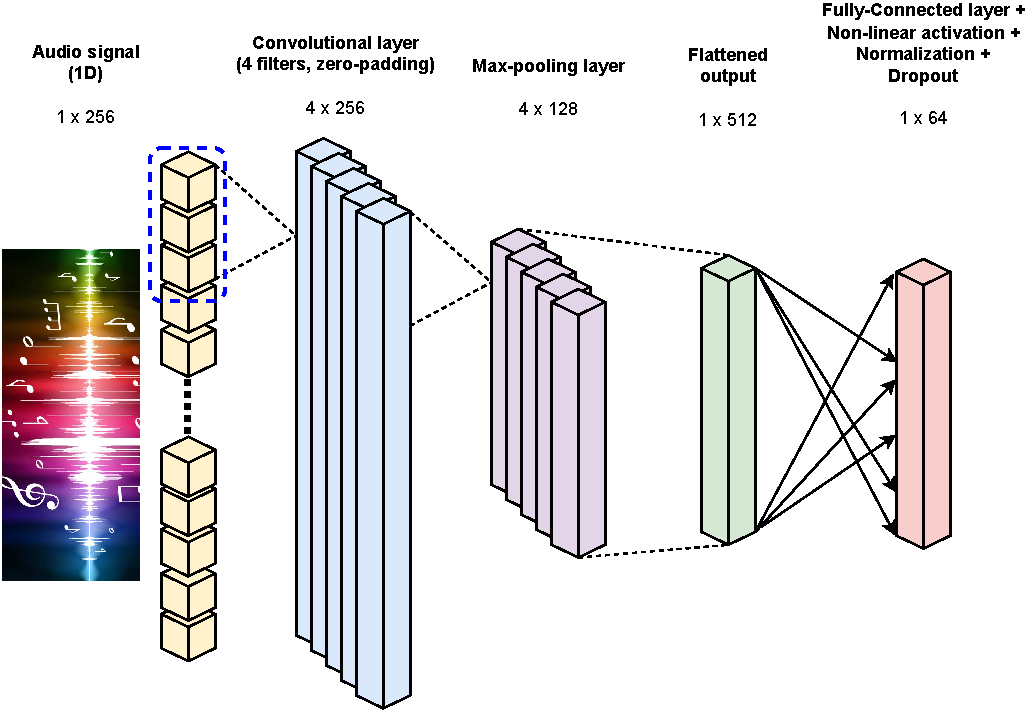
\includegraphics[width=0.8\linewidth]{3_CNN_1D.pdf}
 	\caption{Example of CNN architecture to process 1D-input signals}
 	Source: \textit{Multiclass damage identification in a full-scale bridge using optimally tuned one-dimensional convolutional neural network} \cite{sony2022multiclass}
 	\label{fig:3_CNN_1D}
 \end{figure}
 
Let $x$ be a 1-dimensional input sequence of length $n$, represented as a vector $x = [x_1, x_2, ..., x_n]$. Let $k$ be a filter of length $m$, represented as a vector $k = [k_1, k_2, ..., k_m]$. We can apply the filter $k$ to the input sequence $x$ by computing a convolution operation:

$$(k * x)_i = \sum_{j=1}^m k_j x_{i+j-m}$$

where $*$ denotes the convolution operation, and $i$ ranges from $m$ to $n$. This operation produces a new sequence of length $n - m + 1$, representing the local features extracted from the input sequence $x$ by the filter $k$.

To learn multiple filters and extract different types of features, we use multiple convolutional layers in the network. Each layer applies a set of filters, and produces a set of feature maps. The feature maps can be computed as:

$$h_{i,j} = f(\sum_{k=1}^m W_{j,k} x_{i+k-m} + b_j)$$

where $h$ is the feature map at position $i$ and filter $j$, $W$ is the weight matrix of the $j$-th filter, $b$ is the bias term for the $j$-th filter, and $f$ is an activation function (such as ReLU or sigmoid).

After each convolutional layer, we typically apply a pooling layer to reduce the dimensionality of the features and increase the translation invariance of the network. The most common pooling operation is max pooling, which selects the maximum value within a window of size $p$:

$$y_{i,j} = \max_{k=0}^{p-1} h_{i+k,j}$$

where $y$ is the output of the pooling layer at position $i$ and filter $j$.

Finally, we can use one or more fully connected layers to perform the final classification or regression task. The output of the pooling layer is flattened into a vector, and fed into a set of fully connected layers, with optional dropout regularization and batch normalization:

$$z_j = f(\sum_{i=1}^n W_{i,j} y_i + b_j)$$

where $z$ is the output of the $j$-th fully connected layer, $W$ is the weight matrix, $y$ is the flattened output of the pooling layer, $b$ is the bias term, and $f$ is an activation function. 

\section{Recurrent Neural Networks}
\label{sec:3_rnns}

Recurrent Neural Networks (RNNs) are a type of neural network that are designed to process sequential data, where the order of the input matters. They are widely used in a variety of applications such as natural language processing, speech recognition, image captioning, and time series prediction.

The general theory of RNNs is that they have a feedback loop in their architecture that allows information to be passed from one time step to the next, thereby enabling the network to capture dependencies between the inputs at different time steps. The input at each time step is fed into the network along with the output from the previous time step, and the network uses this information to generate a new output.

There are several types of RNNs, including the basic RNN, the Gated Recurrent Unit (GRU), and the Long Short-Term Memory (LSTM). The basic RNN is the simplest form of RNN, where the output at each time step is a function of the input at that time step and the output from the previous time step. However, it suffers from the vanishing gradient problem, where the gradients become exponentially small as they propagate through time, making it difficult to learn long-term dependencies.

The GRU is a variation of the basic RNN that uses gating mechanisms to control the flow of information through the network. It has fewer parameters than the LSTM and can be faster to train, but it may not perform as well as the LSTM on tasks that require more complex temporal dependencies.

\section{Long Short-Term Memory}
\label{sec:3_LSTMs}

LSTM networks were introduced to address the vanishing gradient problem in standard RNNs. They achieve this by using a memory cell to store information over long periods of time, and three gating mechanisms to control the flow of information through the network.

The three gates are called the input gate, forget gate, and output gate, and they are responsible for deciding which information to store in the memory cell, which information to forget, and which information to output, respectively.

The equations for the input, forget, and output gates are as follows:

\begin{itemize}
	\item Input gate: $i_t &= \sigma(W_i \cdot [h_{t-1}, x_t] + b_i)$
	\item Forget gate: $f_t = sigmoid(W_f * [h_{t-1}, x_t] + b_f)$
	\item Input gate: $o_t = sigmoid(W_o * [h_{t-1}, x_t] + b_o)$
\end{itemize}

Moreover, 

\begin{itemize}
	\item Input gate: $i_t &= \sigma(W_i \cdot [h_{t-1}, x_t] + b_i)$
	\item Forget gate: $f_t = sigmoid(W_f * [h_{t-1}, x_t] + b_f)$
	\item Input gate: $o_t = sigmoid(W_o * [h_{t-1}, x_t] + b_o)$
\end{itemize}

\begin{align*}
	
	\tilde{C}t &= \tanh(W_c \cdot [h{t-1}, x_t] + b_c) \
	C_t &= f_t \cdot C_{t-1} + i_t \cdot \tilde{C}_t \
	h_t &= o_t \cdot \tanh(C_t)
\end{align*}


Here, $x_t$ is the input at time $t$, $h_{t-1}$ is the hidden state from the previous time step, $i_t$ is the input gate activation, $f_t$ is the forget gate activation, and $o_t$ is the output gate activation. $W_i$, $W_f$, and $W_o$ are weight matrices, and $b_i$, $b_f$, and $b_o$ are bias vectors. $\tilde{C}t$ is the candidate value, $C_t$ is the new memory cell value, and $C{t-1}$ is the previous memory cell value. $W_c$ is a weight matrix and $b_c$ is a bias vector.

The memory cell is updated based on the input, forget, and output gates, as well as a new candidate value that is computed based on the current input and hidden state. The equations for the memory cell and candidate value are as follows:

Candidate value: \tilde{C}t = tanh(W_c * [h{t-1}, x_t] + b_c)
Memory cell: C_t = f_t * C_{t-1} + i_t * \tilde{C}_t

Here, \tilde{C}t is the candidate value, C_t is the new memory cell value, and C{t-1} is the previous memory cell value. W_c is a weight matrix and b_c is a bias vector.

Finally, the hidden state at time t is computed based on the output gate and the new memory cell value, using the following equation:

Hidden state: h_t = o_t * tanh(C_t)

This equation scales the memory cell value by the output gate activation, then applies a hyperbolic tangent function to obtain the new hidden state.

In summary, LSTMs use a memory cell and three gating mechanisms to learn long-term dependencies in sequential data. The input, forget, and output gates control the flow of information through the network, while the memory cell stores information over time. The equations for LSTMs involve computing the input, forget, and output gate activations, the candidate value, the new memory cell value, and the new hidden state.

\section{Generative Adversarial Networks}
\label{sec:3_gans}

Throughout most of this book, we have talked about how to make predictions. In some form or another, we used deep neural networks to learn mappings from data examples to labels. This kind of learning is called discriminative learning, as in, we'd like to be able to discriminate between photos of cats and photos of dogs. Classifiers and regressors are both examples of discriminative learning. And neural networks trained by backpropagation have upended everything we thought we knew about discriminative learning on large complicated datasets. Classification accuracies on high-res images have gone from useless to human-level (with some caveats) in just 5-6 years. We will spare you another spiel about all the other discriminative tasks where deep neural networks do astoundingly well.

But there is more to machine learning than just solving discriminative tasks. For example, given a large dataset, without any labels, we might want to learn a model that concisely captures the characteristics of this data. Given such a model, we could sample synthetic data examples that resemble the distribution of the training data. For example, given a large corpus of photographs of faces, we might want to be able to generate a new photorealistic image that looks like it might plausibly have come from the same dataset. This kind of learning is called generative modeling.

Until recently, we had no method that could synthesize novel photorealistic images. But the success of deep neural networks for discriminative learning opened up new possibilities. One big trend over the last three years has been the application of discriminative deep nets to overcome challenges in problems that we do not generally think of as supervised learning problems. The recurrent neural network language models are one example of using a discriminative network (trained to predict the next character) that once trained can act as a generative model.

In 2014, a breakthrough paper introduced Generative adversarial networks (GANs) :cite:`Goodfellow.Pouget-Abadie.Mirza.ea.2014`, a clever new way to leverage the power of discriminative models to get good generative models. At their heart, GANs rely on the idea that a data generator is good if we cannot tell fake data apart from real data. In statistics, this is called a two-sample test - a test to answer the question whether datasets $X=\{x_1,\ldots, x_n\}$ and $X'=\{x'_1,\ldots, x'_n\}$ were drawn from the same distribution. The main difference between most statistics papers and GANs is that the latter use this idea in a constructive way. In other words, rather than just training a model to say "hey, these two datasets do not look like they came from the same distribution", they use the [two-sample test](https://en.wikipedia.org/wiki/Two-sample_hypothesis_testing) to provide training signals to a generative model. This allows us to improve the data generator until it generates something that resembles the real data. At the very least, it needs to fool the classifier even if our classifier is a state of the art deep neural network.

It then applies a function to generate $\mathbf x'=G(\mathbf z)$. The goal of the generator is to fool the discriminator to classify $\mathbf x'=G(\mathbf z)$ as true data, *i.e.*, we want $D( G(\mathbf z)) \approx 1$.
In other words, for a given discriminator $D$, we update the parameters of the generator $G$ to maximize the cross-entropy loss when $y=0$, *i.e.*,

$$ \max_G \{ - (1-y) \log(1-D(G(\mathbf z))) \} = \max_G \{ - \log(1-D(G(\mathbf z))) \}.$$

If the generator does a perfect job, then $D(\mathbf x')\approx 1$, so the above loss is near 0, which results in the gradients that are too small to make good progress for the discriminator. So commonly, we minimize the following loss:

$$ \min_G \{ - y \log(D(G(\mathbf z))) \} = \min_G \{ - \log(D(G(\mathbf z))) \}, $$

which is just feeding $\mathbf x'=G(\mathbf z)$ into the discriminator but giving label $y=1$.


To sum up, $D$ and $G$ are playing a "minimax" game with the comprehensive objective function:

$$\min_D \max_G \{ -E_{x \sim \text{Data}} \log D(\mathbf x) - E_{z \sim \text{Noise}} \log(1 - D(G(\mathbf z))) \}.$$

\subsection{Summary}
\label{subsec:3_gans_summary}

\section{Attention Mechanisms}
\label{sec:3_attention}

\section{Self-Attention and Positional Encoding}
\label{sec:3_self_attention_pos_encoding}

In deep learning, we often use CNNs or RNNs to encode sequences.
Now with attention mechanisms in mind, 
imagine feeding a sequence of tokens 
into an attention mechanism
such that at each step,
each token has its own query, keys, and values.
Here, when computing the value of a token's representation at the next layer,
the token can attend (via its query vector) to each other token 
(matching based on their key vectors).
Using the full set of query-key compatibility scores,
we can compute, for each token, a representation
by building the appropriate weighted sum
over the other tokens. 
Because each token is attending to each other token
(unlike the case where decoder steps attend to encoder steps),
such architectures are typically described as *self-attention* models :cite:`Lin.Feng.Santos.ea.2017,Vaswani.Shazeer.Parmar.ea.2017`, 
and elsewhere described as *intra-attention* model :cite:`Cheng.Dong.Lapata.2016,Parikh.Tackstrom.Das.ea.2016,Paulus.Xiong.Socher.2017`.
In this section, we will discuss sequence encoding using self-attention,
including using additional information for the sequence order.

Given a sequence of input tokens
$\mathbf{x}_1, \ldots, \mathbf{x}_n$ where any $\mathbf{x}_i \in \mathbb{R}^d$ ($1 \leq i \leq n$),
its self-attention outputs
a sequence of the same length
$\mathbf{y}_1, \ldots, \mathbf{y}_n$,
where

$$\mathbf{y}_i = f(\mathbf{x}_i, (\mathbf{x}_1, \mathbf{x}_1), \ldots, (\mathbf{x}_n, \mathbf{x}_n)) \in \mathbb{R}^d$$

according to the definition of attention pooling in
:eqref:`eq_attention_pooling`.
Using multi-head attention,
the following code snippet
computes the self-attention of a tensor
with shape (batch size, number of time steps or sequence length in tokens, $d$).
The output tensor has the same shape.

\section{Graphs}
\label{sec:3_graphs}

% https://arxiv.org/abs/2204.07697
% http://www.deepnlp.org/blog/latex-code-graph-neural-network
% https://towardsdatascience.com/graph-convolutional-networks-deep-99d7fee5706f
% https://www.datacamp.com/tutorial/comprehensive-introduction-graph-neural-networks-gnns-tutorial

A Graph is the type of data structure that contains nodes and edges. A node can be a person, place, or thing, and the edges define the relationship between nodes. The edges can be directed and undirected based on directional dependencies. 

Graphs are excellent in dealing with complex problems with relationships and interactions. They are used in pattern recognition, social networks analysis, recommendation systems, and semantic analysis. Creating graph-based solutions is a whole new field that offers rich insights into complex and interlinked datasets. 

Nevertheless, Graph-based data structures have drawbacks, and researchers must understand them before developing graph-based solutions.

\begin{itemize}
	\item A graph exists in non-euclidean space. It does not exist in 2D or 3D space, which makes it harder to interpret the data. To visualize the structure in 2D space, you must use various dimensionality reduction tools.
	\item Graphs are dynamic; they do not have a fixed form. There can be two visually different graphs, but they might have similar adjacency matrix representations. It makes it difficult for us to analyze data using traditional statistical tools.
	\item Large size and dimensionality will increase the graph's complexity for human interpretations. The dense structure with multiple nodes and thousands of edges is harder to understand and extract insights. 
\end{itemize}

\subsection{Graph Neural Networks}
\label{subsec:3_gnns}

Graph Neural Networks are special types of neural networks capable of working with a graph data structure. They are highly influenced by Convolutional Neural Networks (CNNs) and graph embedding. GNNs are used in predicting nodes, edges, and graph-based tasks. 

\begin{itemize}
	\item A graph exists in non-euclidean space. It does not exist in 2D or 3D space, which makes it harder to interpret the data. To visualize the structure in 2D space, you must use various dimensionality reduction tools.
	\item Graphs are dynamic; they do not have a fixed form. There can be two visually different graphs, but they might have similar adjacency matrix representations. It makes it difficult for us to analyze data using traditional statistical tools.
	\item Large size and dimensionality will increase the graph's complexity for human interpretations. The dense structure with multiple nodes and thousands of edges is harder to understand and extract insights. 
\end{itemize}

\subsection{Graph Neural Networks}
\label{subsec:3_gnns}


\section{Training}
\label{sec:3_training}

Training is the process of iterating through a dataset to make the network learn the optimal mapping (combination of weights) from input to desired output in the data samples. In each iteration, a forward pass through the network is performed, computing the output of each layer until the end. This produces the output response of the network, which is then compared to a desired output with a defined Loss function (L). This function estimates the amount of error, which is back-propagated through the network to update its weights with the aim of minimizing the error. 

Regarding the supervised training paradigm, Backpropagation is an algorithm used for training artificial neural networks (ANNs) used to update the weights and biases of the neurons in the network based on the error between the predicted output and the actual output.

The backpropagation algorithm consists of two phases: the forward pass and the backward pass. During the forward pass, the input is fed into the network and propagated through the layers to obtain the predicted output. During the backward pass, the error between the predicted output and the actual output is computed and used to update the weights and biases of the neurons in the network.

The backpropagation algorithm is based on the chain rule of calculus, which allows the gradient of the loss function with respect to each weight and bias to be computed recursively from the output layer to the input layer of the network. The gradient descent algorithm is then used to update the weights and biases in the direction of the negative gradient of the loss function. In that sense, the main losses used in this work are described throughout the remaining content of this Chapter.

\subsection{Optimizer and learning rate}
\label{subsec:3_optimizer_and_lr}

The ADAM optimizer is a popular optimization algorithm used in deep learning, particularly for training neural networks. It is an adaptive learning rate optimization algorithm that is well suited for large datasets and high-dimensional parameter spaces.

The basic idea behind ADAM is to compute adaptive learning rates for each parameter based on estimates of the first and second moments of the gradients. The algorithm computes a moving average of the gradients and their squared values, and uses these estimates to update the parameters with a learning rate that adapts to the local curvature of the loss function. The algorithm also includes bias-correction terms to ensure that the estimates are unbiased, especially in the early stages of training when the estimates are highly uncertain.

The update rule for ADAM can be expressed mathematically as follows:

\begin{align*}
	m_t &= \beta_1 m_{t-1} + (1-\beta_1) g_t \
	v_t &= \beta_2 v_{t-1} + (1-\beta_2) g_t^2 \
	\hat{m}_t &= \frac{m_t}{1-\beta_1^t} \
	\hat{v}t &= \frac{v_t}{1-\beta_2^t} \
	\theta{t+1} &= \theta_t - \frac{\alpha}{\sqrt{\hat{v}_t}+\epsilon} \hat{m}_t
\end{align*}

Note that the ampersand symbol '&' is used to align the equations at the equal sign, and the double backslash '\' is used to separate the lines of the equation.

where $\theta_t$ is the parameter vector at time step $t$, $g_t$ is the gradient vector, $m_t$ and $v_t$ are the first and second moment estimates at time step $t$, $\hat{m}_t$ and $\hat{v}_t$ are the bias-corrected moment estimates, $\alpha$ is the learning rate, $\beta_1$ and $\beta_2$ are the decay rates for the moment estimates, and $\epsilon$ is a small constant to prevent division by zero.

The algorithm starts with initializing $m_0$ and $v_0$ as zero vectors, and $\theta_0$ as the initial parameter vector. At each iteration, the gradient vector $g_t$ is computed using a batch of training data, and the moment estimates $m_t$ and $v_t$ are updated according to the first two lines of the update rule. The bias-corrected moment estimates $\hat{m}_t$ and $\hat{v}_t$ are then computed using the next two lines of the update rule. Finally, the parameter vector $\theta_t$ is updated using the last line of the update rule.

The hyperparameters $\alpha$, $\beta_1$, $\beta_2$, and $\epsilon$ can be tuned to optimize performance on a particular dataset and neural network architecture.

On the other hand, The learning rate is a key hyperparameter in the optimization process of machine learning algorithms, including optimizer updates like the ADAM optimizer. The learning rate controls the step size taken in the direction of the negative gradient during each iteration of the optimization process.

If the learning rate is too small, the optimization process will be slow and may get stuck in local minima. On the other hand, if the learning rate is too large, the optimization process may overshoot the minimum and oscillate back and forth, or even diverge.

In the context of the ADAM optimizer, the learning rate is used to adjust the size of the update step taken in the direction of the estimated gradient. The update step is multiplied by the learning rate, which determines the size of the step. A larger learning rate will result in larger update steps, and a smaller learning rate will result in smaller update steps.

In practice, the learning rate is usually set through a process called hyperparameter tuning, where different values of the learning rate are tried on a validation set to find the optimal value that results in the best performance of the model on the test set.

One common technique to adjust the learning rate during training is called learning rate scheduling. This involves decreasing the learning rate over time, often according to a predetermined schedule or based on the performance of the model on a validation set. This technique can help improve the convergence and stability of the optimization process, particularly in the later stages of training when the model is close to the optimal solution.

Overall, the learning rate plays a crucial role in the optimization process of machine learning algorithms, including optimizer updates like the ADAM optimizer. Selecting an appropriate learning rate is important for achieving fast and stable convergence to the optimal solution.

\subsection{Regression losses}
\label{subsec:3_regression_losses}

% https://blmoistawinde.github.io/ml_equations_latex/

A regression loss is a type of loss function used in regression problems to measure the difference between the predicted and true values of a continuous variable. In other words, it is a way to quantify how well a machine learning model is able to predict numerical values based on input data.

In regression problems, the goal is to learn a function that maps input features to output values. A regression loss is used to train the model by penalizing the difference between the predicted and true output values. The loss function is typically minimized during training, so that the model learns to make more accurate predictions. There are several types of regression loss functions, such as the Quantile loss, Log-Cosh or Mean Absolute Error (MAE). In this work we mainly focus on the Mean Square Error (MSE) and SmoothL1, also known as Huber loss.

\subsubsection{Mean Square Error loss}
\label{subsubsec:3_mse_loss}

The Mean Squared Error (MSE) loss is a commonly used loss function in regression problems. It measures the average squared difference between the predicted and true values of a continuous variable. The MSE loss is given by:

\begin{equation}
	MSE(y, \hat{y}) = \frac{1}{n}\sum_{i=1}^{n}(y_i - \hat{y_i})^2
\end{equation}

where $y_i$ is the true value of the $i$-th data point, $\hat{y_i}$ is the predicted value, and $n$ is the number of data points.

The MSE loss penalizes large errors more strongly than small errors, since it uses the square of the difference between the predicted and true values. This makes it sensitive to outliers and can lead to overfitting if the data contains extreme values.

The MSE loss is used in many regression problems, such as linear regression, polynomial regression, and neural networks. It is often used as a performance metric to evaluate the quality of the model's predictions.

\subsubsection{SmoothL1 loss}
\label{subsubsec:3_smoothL1_loss}

SmoothL1 loss, also known as Huber loss, is a loss function used in regression problems to measure the difference between the predicted and true values of a continuous variable. It is a variant of the L1 loss that is less sensitive to outliers and has a smooth gradient near zero.

The SmoothL1 loss function can be defined as follows:

\begin{equation}
	L(y, \hat{y}) = \begin{cases}
		\frac{1}{2}(y - \hat{y})^2 & \text{if } |y - \hat{y}| < 1 \
		|y - \hat{y}| - \frac{1}{2} & \text{otherwise} \
	\end{cases}
\end{equation}

where $y$ is the true value, $\hat{y}$ is the predicted value, and $|\cdot|$ represents the absolute value function.

The SmoothL1 loss function behaves like the L1 loss for small errors and like the L2 loss for large errors. Specifically, for errors smaller than 1, it uses the squared difference between the predicted and true values, which has a smooth gradient. For larger errors, it uses the absolute difference, which is less sensitive to outliers than the squared difference.

The SmoothL1 loss is used in regression problems when the data contains outliers or when the model needs to be less sensitive to large errors. It is commonly used in object detection and localization tasks, where the predicted bounding boxes can be highly sensitive to small changes in the input data.

\subsection{Softmax loss}
\label{subsec:3_softmax_loss}

The softmax loss, also known as the cross-entropy loss, is a commonly used loss function in classification problems. It measures the difference between the predicted probability distribution and the true probability distribution of a categorical variable. The softmax loss is given by:

\begin{equation}
	CE(y, \hat{y}) = -\frac{1}{n}\sum_{i=1}^{n}\sum_{j=1}^{k} y_{i,j}\log(\hat{y_{i,j}})
\end{equation}

where $y_{i,j}$ is the true probability of the $i$-th data point belonging to class $j$, $\hat{y_{i,j}}$ is the predicted probability, $n$ is the number of data points, and $k$ is the number of classes.

The softmax function is applied to the output of the model to obtain a probability distribution over the classes. The predicted probability of class $j$ is given by:

\begin{equation}
	\hat{y_{i,j}} = \frac{e^{z_{i,j}}}{\sum_{l=1}^{k} e^{z_{i,l}}}
\end{equation}

where $z_{i,j}$ is the unnormalized score or logit for class $j$ of the $i$-th data point.

The softmax loss penalizes the model more heavily for predictions that are far from the true probabilities. It encourages the model to assign higher probabilities to the correct classes and lower probabilities to the incorrect classes.

The softmax loss is used in many classification problems, such as image classification, natural language processing, and speech recognition. It is often used as a performance metric to evaluate the quality of the model's predictions.

\subsection{Negative Log-Likelihood loss}
\label{subsec:3_NLL_loss}

Negative Log Likelihood (NLL) loss is a loss function commonly used in classification problems, particularly in deep learning models that output probabilities for each class. It is a type of maximum likelihood estimation (MLE) loss, which means it attempts to maximize the likelihood of the predicted probabilities given the true labels.

The NLL loss function can be defined as follows:

\begin{equation}
	L(y_i, \hat{y_i}) = -\log(\hat{y_{i,y_i}})
\end{equation}

where $y_i$ is the true label of the $i$-th data point, $\hat{y_i}$ is the predicted probability distribution for that point, and $\hat{y_{i,y_i}}$ is the predicted probability for the true label.

The NLL loss penalizes the model for assigning low probabilities to the true label, while rewarding it for assigning high probabilities. It is a logarithmic loss function, which means that the penalty for low probabilities increases exponentially as the predicted probability approaches zero.

The NLL loss is used in classification problems because it provides a gradient that can be used to update the model parameters during training, in order to improve the accuracy of the predicted probabilities. It is commonly used in conjunction with softmax activation function, which ensures that the predicted probabilities sum to one across all classes.

\subsection{Winner-Takes-All loss}
\label{subsec:3_WTA_loss}

Winner-Takes-All (WTA) loss is a loss function used in clustering problems, particularly in competitive learning models. It is a type of unsupervised learning, which means that it does not require labeled data for training.

The WTA loss function can be defined as follows:

\begin{equation}
	L(y_i, f(x_i)) = \begin{cases}
		0 & \text{if } y_i = \arg\max_j f_j(x_i) \
		1 & \text{otherwise} \
	\end{cases}
\end{equation}

where $y_i$ is the true cluster of the $i$-th data point, $f_j(x_i)$ is the activation of the $j$-th neuron in the output layer for that point, and $\arg\max_j f_j(x_i)$ is the index of the neuron with the highest activation.

The WTA loss function penalizes the model for assigning a data point to the wrong cluster. It works by forcing each neuron in the output layer to specialize in a particular cluster, such that the neuron with the highest activation for a given point corresponds to the true cluster of that point.

The WTA loss is used in clustering problems because it encourages the model to learn a set of representative clusters that capture the structure of the data, without requiring any prior knowledge of the true labels. It is commonly used in conjunction with competitive learning algorithms, such as self-organizing maps (SOMs), that use local competition between neurons to learn a topology-preserving mapping from the input space to the output space.

\subsection{Hinge loss}
\label{subsec:3_hinge_loss}

Hinge loss is a loss function used in classification problems, particularly in support vector machines (SVMs). It is a type of max-margin loss, which means it attempts to maximize the margin between the decision boundary and the data points.

The hinge loss function can be defined as follows:

\begin{equation}
	L(y_i, f(x_i)) = \max(0, 1 - y_i f(x_i))
\end{equation}

where $y_i$ is the true label of the $i$-th data point, $f(x_i)$ is the predicted score for that point, and $1$ is a margin hyperparameter that determines the width of the margin.

If $y_i f(x_i) \geq 1$, then the point is correctly classified and the loss is zero. If $y_i f(x_i) < 1$, then the point is misclassified and the loss is proportional to the distance between the predicted score and the correct score. The loss function penalizes misclassifications linearly, with a slope of -1 for negative misclassifications and 0 for positive misclassifications.

The hinge loss is used in SVMs because it encourages the model to find a decision boundary that maximizes the margin between the classes, while still correctly classifying the data points. This results in a more robust and generalizable model.

\subsection{Regularization techniques}
\label{subsec:3_regularization}

Regularization techniques in deep learning are used to prevent overfitting and improve the generalization performance of a model. Overfitting occurs when a model fits the training data too closely and captures noise or irrelevant patterns, resulting in poor performance on new, unseen data. Here are some commonly used regularization techniques in deep learning:

L1 and L2 regularization: L1 and L2 regularization are two popular regularization techniques that add a penalty term to the loss function during training. L1 regularization adds the sum of the absolute values of the weights to the loss function, while L2 regularization adds the sum of the squares of the weights. This encourages the model to learn simpler and more generalizable representations by shrinking the weights towards zero.

Dropout: Dropout is a regularization technique that randomly drops out some units (neurons) in a layer during training. This forces the remaining units to learn more robust and diverse representations that generalize better to new data. Dropout has been shown to be effective in reducing overfitting, particularly in deep neural networks with many layers.

Data augmentation: Data augmentation is a technique that artificially increases the size of the training set by generating new examples from existing ones. This can be done by applying transformations such as rotations, translations, flips, or adding noise to the input data. Data augmentation can help reduce overfitting by increasing the diversity of the training data and improving the generalization performance of the model.

Early stopping: Early stopping is a technique that monitors the performance of the model on a validation set during training and stops the training process when the performance starts to degrade. This prevents the model from overfitting to the training data and allows it to generalize better to new data.

Batch normalization: Batch normalization is a technique that normalizes the activations of a layer by subtracting the batch mean and dividing by the batch standard deviation. This helps stabilize the distribution of the activations and reduces the internal covariate shift, which can improve the training process and reduce overfitting.

Weight decay: Weight decay is a technique that adds a penalty term to the loss function during training, similar to L2 regularization. The penalty term is proportional to the square of the weights, and it encourages the model to learn smaller and simpler weights, which can reduce overfitting.

These are some of the commonly used regularization techniques in deep learning. They can be combined and tuned to improve the performance of a model on a specific task and dataset.

Moreover, another interesting technique to help the model improve during training is hard-mining. Hard-mining is a technique in deep learning used to improve the training of a model by focusing on the samples that are most difficult to classify correctly.

During training, the model makes predictions on a batch of training data, and the loss function is computed based on the difference between the predicted values and the true values. In hard-mining, the training samples that contribute the most to the loss function are identified, and these samples are given more importance during training.

The idea behind hard-mining is that by focusing on the difficult samples, the model is forced to learn more discriminative features that can better distinguish between the different classes. This can lead to better generalization performance and improved accuracy on the test data.

There are several ways to implement hard-mining in deep learning, including:

Hard negative mining: This involves selecting the training samples that are misclassified with the highest confidence by the model and including them in the next batch of training data. By focusing on the difficult negative samples, the model can learn to better distinguish between the different classes and reduce the number of false negatives.

Hard positive mining: This involves selecting the training samples that are misclassified with the lowest confidence by the model and including them in the next batch of training data. By focusing on the difficult positive samples, the model can learn to better distinguish between the different classes and reduce the number of false positives.

Curriculum learning: This involves gradually increasing the difficulty of the training data over time. The model is first trained on easy samples and then gradually exposed to more difficult samples. This can help the model learn more robust and generalizable features by gradually increasing the complexity of the training data.

Overall, hard-mining is a useful technique in deep learning for improving the training of a model by focusing on the difficult samples. By incorporating hard-mining into the training process, the model can learn more discriminative features and improve its generalization performance on new, unseen data.